%\graphicspath{{/figuras}}
\chapter{Introdu\c{c}ão}

%The methods used to search for periodicity in astronomical time
%series may be divided into two groups: Fourier techniques and
%phase-diagram analyses. The first group includes the classical
%Fourier transform, and its variations introduced to deal with
%unevenly sampled data. The second one is based on the analysis of the dispersion of the light curve, observed data folded over a trial period as a function of phase, for a set of trial periods.

Na astronomia, especialmente no campo das estrelas variáveis, geralmente é necessário analisar dados com períodos desconhecidos. Existem métodos desenvolvidos para lidar com dados que possuem intervalos espaciais uniformes, porém as observações geralmente são limitadas para o período da noite e possuem limitações devido ao clima e disponibilidade do telescópio, o que faz com que os dados sejam espaçados por uma ordem de horas, dias ou até mesmo meses \citep{mello81}. 
%Assim, os dados obtidos raramente são igualmente espaçados.
Assim, os dados obtidos raramente possuem um espaçamento constante entre os pontos de observação e lidar com este tipo de série temporal não é um trabalho fácil \citep{lomb}.

%Ao trabalhar com estrelas variáveis, que são estrelas em que o seu brilho aparente varia em função do tempo, podemos obter o período de variação da magnitude  através da curva de luz da estrela, ou seja, a partir dos dados observacionais obtidos pelos telescópios. A obtenção deste período de oscilação da luz de uma estrela variável é fundamental para descrever a estrela, pois podemos relacionar este periodo com luminosidade (\textcolor{red}{(citar a henrietta)}, densidade (\textcolor{red}{(citar a relação periodo-densidade)}, cor (\textcolor{red}{(citar a relacão com a cor)}, etc... (\textcolor{red}{(ver o que mais podemos calcular, talvez metalicidade...)}% Através do seu período podemos estimar os valores de luminosidade, massa, distância, densidade, etc.

Estrelas variáveis são objetos em que seu brilho aparente oscila em função do tempo. A partir desta variação do brilho, podemos obter o período de variação na magnitude da estrela analisando a sua curva de luz, ou seja, examinando os dados observacionais obtidos pelo telescópio. A obtenção deste período de oscilação da luz de uma estrela variável é fundamental para descrever a estrela, pois podemos relacionar este período com luminosidade \citep{Leavitt1912}, densidade \citep{Payne1930} e cor \citep{Kraft1960}. Também, as estrelas variáveis são utilizadas como velas padrões e através da relação entre período-luminosidade podemos estimar distâncias astronômicas, que é um dos problemas fundamentais da astronômia.
%, etc... (\textcolor{red}{(ver o que mais podemos calcular, talvez metalicidade...)}).



Existem diversos algoritmos para a determinação de períodos em dados astronômicos. Cada um possui um método diferente ou alguma pequena modificação em relação aos demais. Mesmo com uma grande quantidade de métodos, nenhum deles parece se sobressair de uma forma geral \citep{comparison}. Alguns métodos são melhores para lidar com dados que sejam igualmente espaçados, enquanto que outros são adaptados para lidar com espaçamento variável. Os algoritmos mais utilizados para determinação de períodos em séries temporais astronômicas fazem um ajuste de curva utilizando o método dos mínimos quadrados \citep{lomb} ou utilizam análise de Fourier \citep{mello81}. Outros métodos tentam minimizar alguma grandeza na dispersão da série temporal no espa\c{c}o de fase, como é o caso da análise de variância \citep{aov} e da entropia \citep{entropy}.

%Como dito anteriormente, cada método possui certas vantagens e disvantagens. Por exemplo, a analise de Fourier é eficiente e rápida, porém não é muito sensitiva para para fun\c{c}ões não senoidais

%Each method has certain advantages and disadvantages. For example, while Fourier analysis is faster and extremely efficient, it is much less sensitive to non-sinusoidal functions than the phase-diagram analysis. Also, phase-diagram methods are less affected by randomly occurring gaps in the data, provided that the coverage of the light curve is reasonably uniform in phase space.

O objetivo deste trabalho é testar um algoritmo que seja confiável para trabalhar com séries temporais astronômicas e que não seja dependente do espaçamento entre os dados observacionais. Este algoritmo trabalha com a entropia de Shannon condicional \citep{ce, Cincotta1999}, um método que utiliza a dispersão no espaço de fase para obter o período da série temporal através da minimização da entropia.

%A ideia deste projeto é testar um método para determinar multiplos períodos de pulsa\c{c}ão de estrelas variáveis, tendo em vista que nenhum destes métodos são aplicados diretamente para esta fun\c{c}ão. Este método, chamado de Entropia Condicional, busca a minimiza\c{c}ão da entropia de Shannon condicional na dispersão da série temporal no espa\c{c}o de fase.
%In this paper, we present a phase-diagram analyses method called Conditional Entropy method. The idea is develop a fast and reliable method to work with variable stars.

%Neste capítulo de introdução será feita uma revisão de alguns tópicos de astrofísica estelar importantes para a compreensão do trabalho. No capítulo \ref{cap:estrelas} será abordado o tópico sobre estrelas variáveis, explicando a sua história, classificação e importância. Uma breve explicação das principais técnicas, dando ênfase para a entropia de Shannon, será vista no capítulo \ref{cap:tecnicas}. Finalmente, os resultados obtidos e uma discussão será abordada no capítulo \ref{cap:resultados}.

Neste capítulo de introdução será feita uma revisão de alguns tópicos de astrofísica estelar importantes para a compreensão do trabalho e uma revisão história e bibliográfica sobre as estrelas variáveis, técnicas de observação e métodos e detecção de períodos. No capítulo \ref{cap:estrelas} será abordado o tópico sobre estrelas variáveis, explicando a sua classificação, importância e as principais relações com o período. A explicação do método utilizado neste trabalho será abordado no capítulo \ref{cap:tecnicas}. Finalmente, os resultados obtidos e exemplo de aplicação do método será discutida no capítulo \ref{cap:resultados}.



\section{Conceitos de astrofísica estelar}

%\nocite{keplerLivro2013}
\nocite{karttunenLivro}

\subsection{Fluxo}

O Fluxo ($F$) é a medida de energia por unidade de área e por unidade de tempo, ou seja, é a potência emitida através de uma superfície. O fluxo a uma distância $r$ de uma estrela é obtido pela expressão,
\begin{align}
F(r) = \frac{L}{4\pi r^2} \quad \left[ \si{W.m^{-2}}\right] \,\, \text{ou} \,\, \left[\si{erg.cm^{-2}.s^{-1}}\right] \label{eq:fluxo}
\end{align}
em que $L$ é a luminosidade da estrela ou a energia total emitida por unidade de tempo em todas as direções. Pela expressão do fluxo, podemos perceber que esta quantidade diminui com o quadrado da distância.

\subsection{Magnitude}

O sistema de magnitude foi criado pelo Grego Hiparco (160-125 a.C.) há mais de 2000 anos. Ele dividiu as estrelas visíveis a olho nu de acordo com o seu brilho aparente, classificando as estrelas mais brilhantes como magnitude 1 ($m=1$) e as mais fracas como magnitude 6 ($m=6$). Como a percepção de brilho do olho humano é logarítmica, o fluxo de uma estrela com 
$m=1$ é 100 vezes mais brilhante que uma estrela com $m=6$. Por definição, a magnitude aparente ($m$) ou brilho aparente, é a medida do brilho de um objeto observado na Terra que é dado por,
\begin{align}
m = - 2,5 \log \frac{F}{F_0}
\end{align}
em que $F_0$ é fluxo para magnitude $m=0$. Para duas estrelas com magnitudes $m_1$ e $m_2$, e fluxos $F_1$ e $F_2$, a sua diferença é expressa pela relação,
\begin{align}
m_2 - m_1 = -2,5 \log \frac{F_2}{F_1}.
\end{align}
A tabela \ref{tab:magnitudes} possui uma comparação entre as magnitudes aparentes de alguns objetos celestes.

\begin{table}[h!]
\begin{center}
\captionof{table}{Exemplo de magnitudes aparentes.}
\begin{tabular}{c|c} 
\hline 
Objeto & Magnitude \\ 
\hline 
Vega & 0 \\ 
Sírius & -1,46 \\
Marte & -2,0 \\
Júpiter & -2,7 \\ 
Lua Cheia & -12,8 \\
Sol & -26,74 \\
\hline 
\end{tabular} \\
\small
\vspace{2mm}Fonte: Extraído de \cite{keplerLivro2013}.
\label{tab:magnitudes}
\end{center}
\end{table}

\subsection{Magnitude absoluta e o módulo de distância}

A magnitude aparente é uma medida de brilho que depende da distância e por isso não representa exatamente o brilho real de uma estrela. Para podermos comparar o brilho de duas estrelas, precisamos de uma medida que seja independente da distância. Assim, a magnitude absoluta ($M$) representa o brilho da estrela a uma distancia de 10 parsecs da Terra.
\begin{align}
M = -2,5 \log \frac{F(10\si{pc})}{F_0}
\end{align}
A diferença entre a magnitude aparente e absoluta é dada por,
\begin{align}
m - M &= - 2,5 \log \frac{F}{F_0} + 2,5 \log \frac{F(10\si{pc})}{F_0} \\
&= -2,5 \left[ \log \frac{F}{F_0} - \log \frac{F(10\si{pc})}{F_0} \right] \\
&= -2,5 \log \left[ \frac{F}{F_0} \frac{F_0}{F(10\si{pc})} \right] \\
&= -2,5 \log \frac{F}{F(10\si{pc})} \label{eq:mag_abs_incompleto}
\end{align}
mas de acordo com a expressão \eqref{eq:fluxo} para o fluxo,
\begin{align}
\frac{F}{F(10\si{pc})} = \frac{L}{4\pi r^2} \frac{4\pi \left(10 \si{pc}\right)^2}{L} = \frac{100 \si{pc}^2}{r^2}
\end{align}
em que $r$ é a distância da estrela. Substituindo este resultado na equação \eqref{eq:mag_abs_incompleto},
\begin{align}
m - M &= -2,5 \log \frac{100 \si{pc}^2}{r^2} \\
&= -2,5 \log 100 \si{pc}^2 + 2,5 \log r^2 \\
&= 5 \log r - 5
\end{align}
e definindo o módulo de distância $\mu$ como,
\begin{align}
\mu = m - M
\end{align}
obtemos a expressão,
\begin{align}
\mu = m - M = 5 \log r - 5 \label{eq:modulo_distancia}
\end{align}
lembrando que a distância $r$ deve ser medida em parsecs. Evidenciando $r$, obtemos uma expressão para calcular a distância,
\begin{align}
r = 10^{0,2\left( m - M + 5 \right)} \quad \text{ou} \quad  r = 10^{0,2\left( \mu + 5 \right)} \quad \left[ \si{pc} \right].
\end{align}

\subsection{Sistemas de magnitudes}

A magnitude aparente $m$ que observamos nos telescópios depende do detector utilizado, do filtro aplicado e das configurações do telescópio. Geralmente a sensibilidade de um detector não é a mesma para diferentes comprimentos de onda. Assim, o fluxo medido pelo equipamento é uma parcela do fluxo total da estrela. Portanto, sistemas de magnitudes foram desenvolvidos. Estes sistemas são conjuntos de filtros que permitem o equipamento coletar apenas uma determinada faixa de comprimento de onda. Um dos sistemas mais utilizados é o conjunto UBV (ultravioleta, azul e visível) desenvolvido por \citet{Johnson1953}. Alguns anos mais tarde, \citet{Cousins1973} adaptou o trabalho de Johnson para o hemisfério sul. Outro conjunto comumente utilizado é o sistema UBVRIJKL \citep{Johnson1966}. A tabela \ref{tab:filtros} mostra o comprimento de onda efetivo $\lambda_{eff}$ e a largura de banda $\Delta \lambda$ de alguns filtros utilizados na detecção de fluxo.

\begin{table}[h!]
\begin{center}
\captionof{table}{Filtros, comprimento de onda efetivo e largura da banda.}
\begin{tabular}{c|c|c} 
\hline 
Cor & $\lambda_{eff}$ ($\si{\nano\metre}$) & $\Delta \lambda$ ($\si{\nano\metre}$) \\ 
\hline 
U & 366 & 65 \\ 
B & 436 & 89\\
V & 545 & 84 \\
R & 641 & 158\\ 
I & 798 & 154 \\
%J & 1,2 \si{\micro\metre} \\
%H & 1,6 \si{\micro\metre}\\
%K & 2,1 \si{\micro\metre}\\
\hline 
\end{tabular} \\
\small
\vspace{2mm}Fonte: Extraído de \cite{Catelan_book}.
\label{tab:filtros}
\end{center}
\end{table}


\subsection{Magnitude bolométrica}

Em um caso ideal, seria possível medir todo o espectro magnético em um único aparelho. Essa medida seria a \textit{magnitude bolométrica}. Infelizmente, é difícil realizar esta medida pois a nossa atmosfera absorve parte da radiação e também precisamos de diferentes detectores para determinadas frequências.

A magnitude bolométrica ($m_{\si{bol}}$) pode ser obtida pela magnitude visual ($m_V$),
\begin{align}
m_{\si{bol}} = m_V - BC
\end{align}
em que $BC$ é a correção bolométrica. Por definição, esta correção possui valor zero para estrelas parecidas com o nosso Sol e possui valores maiores para estrelas mais quentes ou mais frias do que o Sol.

\subsection{Extinção atmosférica}

A nossa atmosfera não é inteiramente transparente. Embora permita a passagem de luz visível, a atmosfera absorve radiação ultravioleta e várias bandas do infravermelho. Também, existem diversas moléculas que desviam a luz em todas as direções e absorvem parte da radiação reemitindo em praticamente todos os comprimentos de onda. Toda essa perda em radiação devida aos constituintes da atmosfera é chamada de \textit{extinção atmosférica}. Quanto maior a quantidade de ar atravessada pela luz, maior a extinção. Este é um dos motivos que os telescópios terrestres são localizados em lugares altos como montanhas.

Para corrigir este efeito, a magnitude observada em um determinado comprimento de onda pode ser escrita como,
\begin{align}
m_{\lambda} = m_{\lambda_0} + K_{\lambda} \cdot X
\end{align}
em que $m_{\lambda_0}$ é a magnitude em um determinado comprimento de onda no alto da atmosfera, $K_{\lambda}$ é o coeficiente de extinção e $X$ é a massa de ar, que depende do ângulo de observação.

\subsection{Extinção interestelar}

Devido a presença de poeira no meio interestelar, parte da radiação emitida por alguma fonte é absorvida, desviada e geralmente reemitida em outro comprimento de onda. Toda a perda de radiação devido ao meio interestelar é chamada de \textit{extinção interestelar}. Este desvio que ocorre na radiação causa um desvio para o vermelho no espectro de frequência da luz. Por causa disto, devemos fazer uma correção na formula \eqref{eq:modulo_distancia} da magnitude aparente observada.

Sendo a extinção interestelar representada pela letra $A_{\lambda}$ com um subscrito indicando a banda espectral, a correção na magnitude absoluta para um determinado comprimento de onda a uma distância $r$ será,
\begin{align}
m_{\lambda} - M_{\lambda} - A_{\lambda} = 5 \log r - 5 \\
M_{\lambda} = m_{\lambda} - A_{\lambda} - 5 \log r + 5.
\end{align} 
e da mesma forma, a correção para o calculo da distância será,
\begin{align}
r = 10^{0.2 \left(m -M + 5 - A_{\lambda} \right)}.
\end{align}

%\subsection{Índice de Cor}

%\subsection{Diagrama H-R}
 
\subsection{Data Juliana}

%livro do catelan, capitulo 2
A data Juliana (sigla JD) foi proposta por Josephus Justus Scalinger em 1583. Com esta data é possível calcular facilmente o intervalo de tempo entre um evento astronômico e outro, pois este formato de medir tempo não possui meses e nem anos, apenas mede a quantidade de dias solares médios decorridos desde 1 de Janeiro de 4713 a.C. (início da era Juliana).


\subsection{Curva de luz}

%livro do catelan, capitulo 2
A curva de luz de uma estrela é simplesmente o gráfico de sua magnitude aparente versus tempo, ou seja, um gráfico dos dados obtidos pelo telescópio, como mostra a figura \ref{fig:curva_luz}. A partir desses dados que os métodos de detecção de período operam e, no momento em que se define o período da estrela, é possível construir a curva de luz no espaço de fase, como será visto a seguir.

\begin{figure}[h!]
\centering
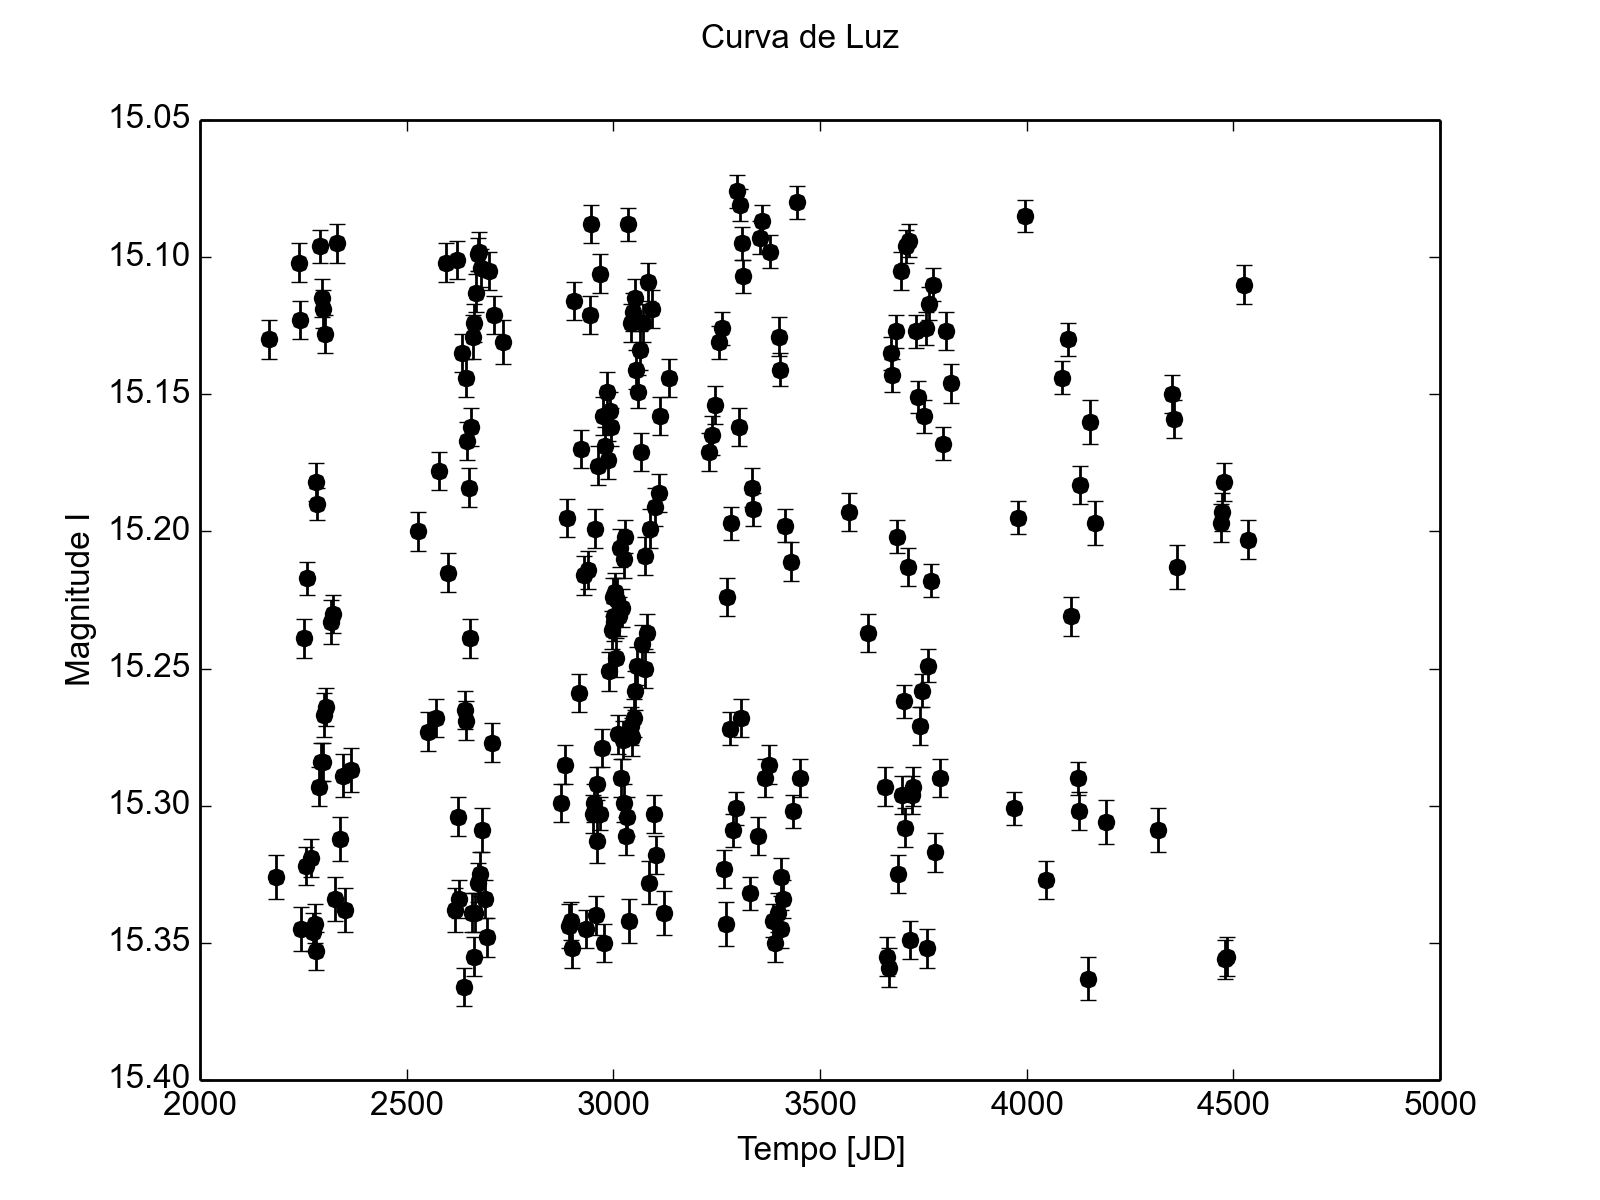
\includegraphics[width=0.7\linewidth]{0018_curva.png}
\caption[Exemplo de curva de luz]{Exemplo de curva de luz utilizando a Cefeida OGLE-LMC-CEP-0018 do catálogo OGLE. Podemos perceber o espaçamento entre os conjuntos de pontos.}
\label{fig:curva_luz}
\end{figure}


\subsection{Fase e o Espaço de Fase}

Quando uma estrela possui um comportamento periódico, a variação em sua magnitude é representada em ciclos iguais. Cada ciclo é uma fase. Se os ciclos são iguais, não importa qual ciclo nós estamos observando, apenas onde nós estamos no ciclo. Com isso, o espaço de fase é uma representação de todos os ciclos observados em apenas uma fase, ou em apenas um ciclo. Desta forma, os pontos de sobrepõem e formam uma oscilação geral da estrela. A fase é calculada pela seguinte expressão,
\begin{equation}
\phi_i = \frac{t_i}{P} - \Big[\frac{t_i}{P}\Big]
\end{equation}
em que $t_i$ é o i-ésimo dado do tempo, $P$ é o período de oscilação da magnitude e a quantidade entre colchetes representa apenas o numero inteiro da divisão. O espaço de fase é o gráfico da magnitude aparente versus a fase.


\begin{figure}[h!]
\centering
\begin{subfigure}{.5\textwidth}
  \centering
  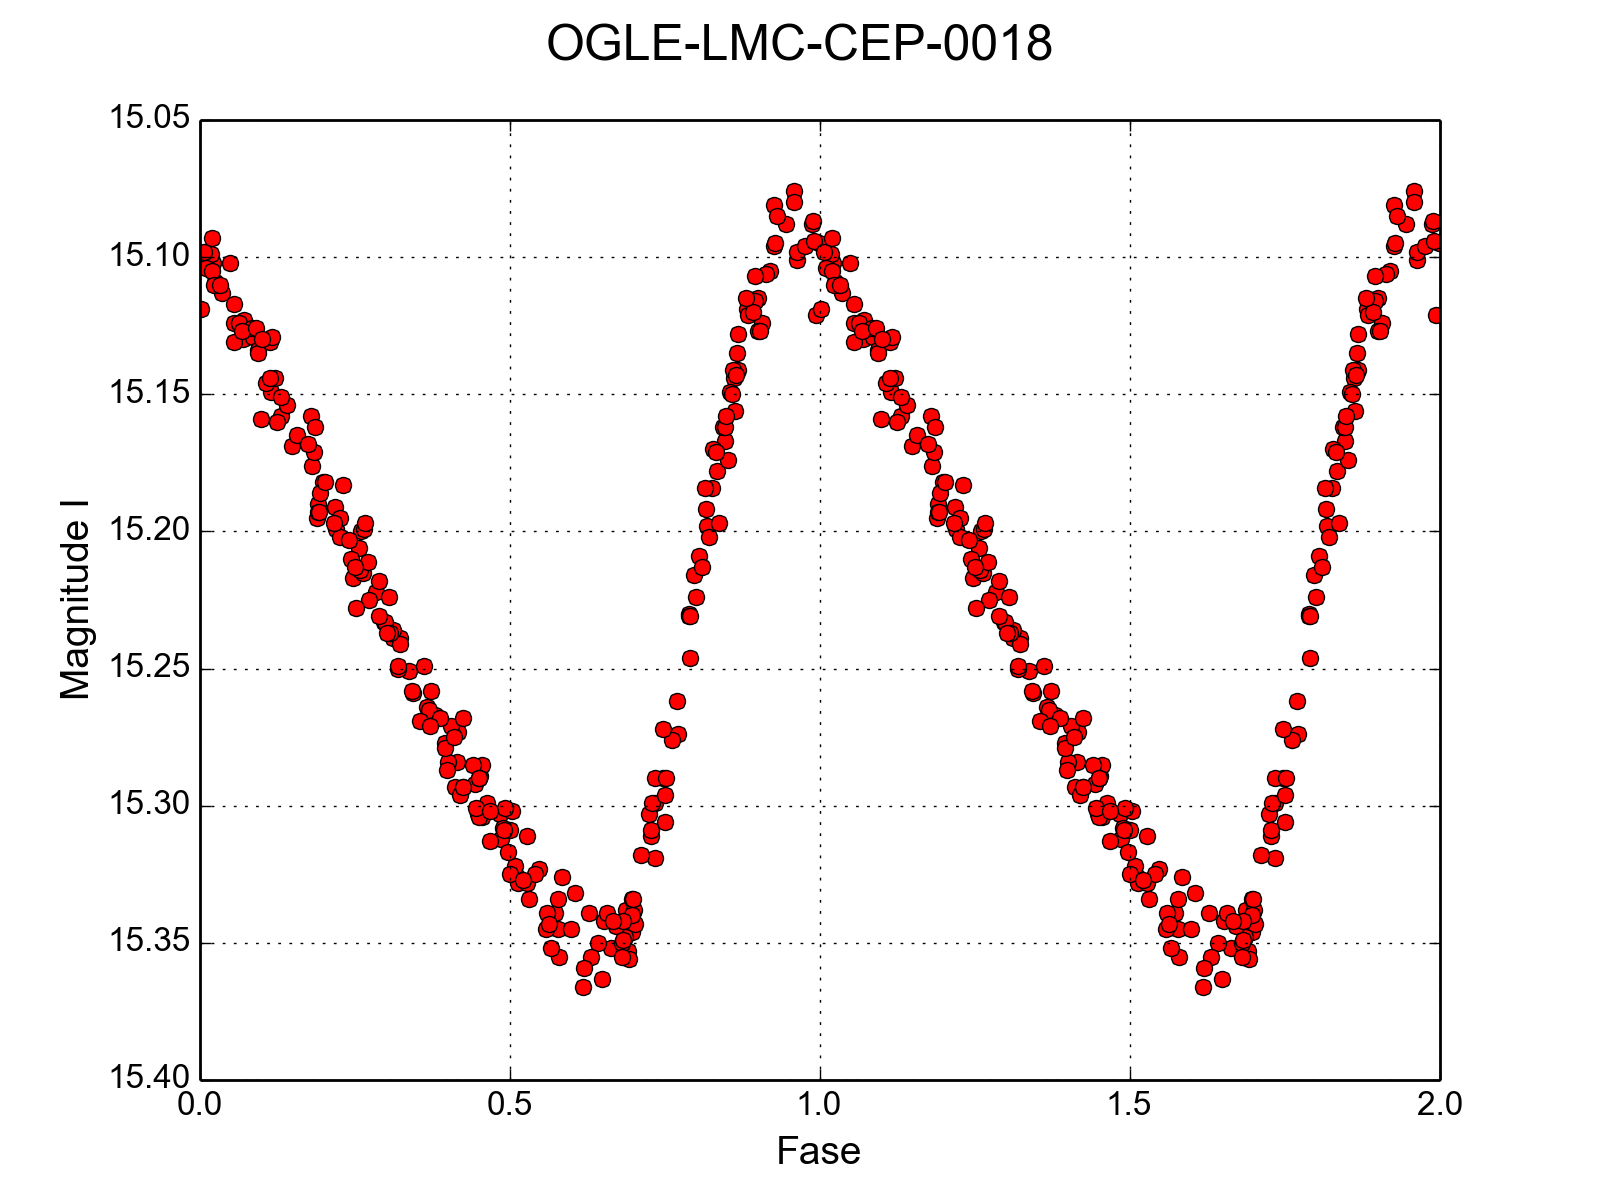
\includegraphics[width=\linewidth]{0018_correct.png}
  \caption{Período correto}
  \label{fig:right}
\end{subfigure}%
\begin{subfigure}{.5\textwidth}
  \centering
  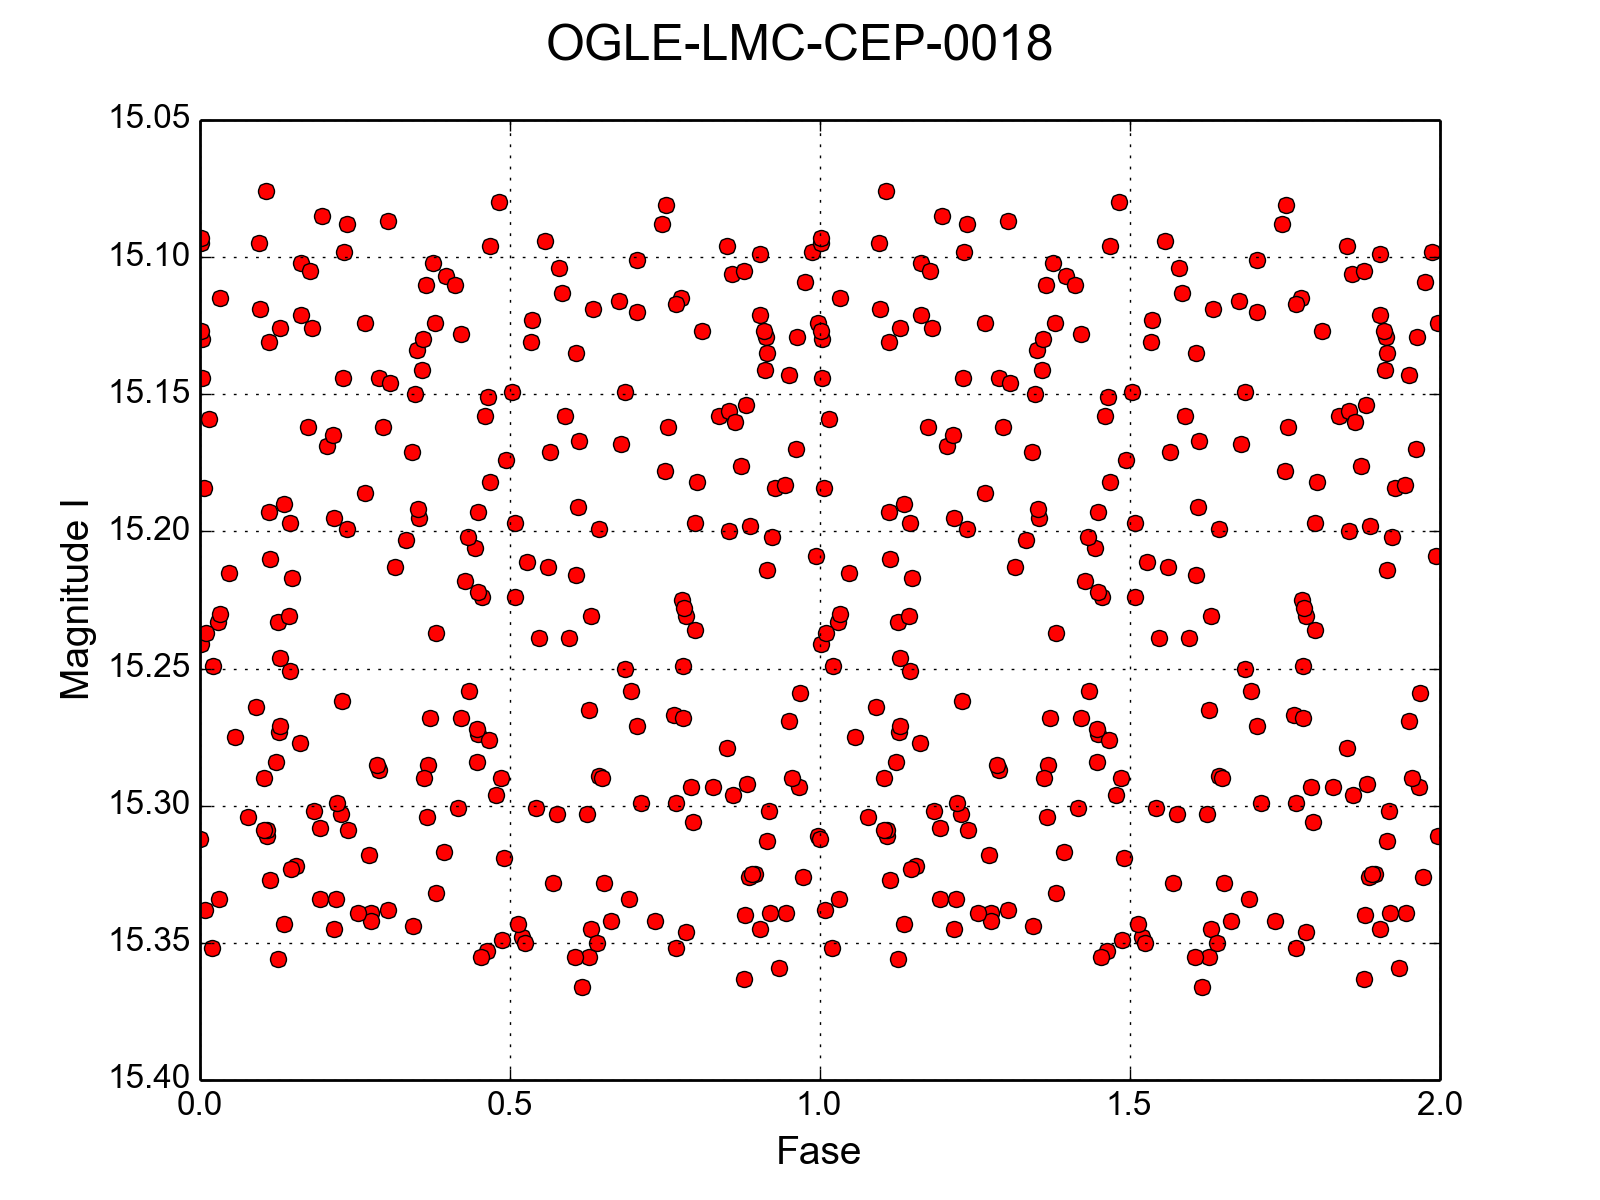
\includegraphics[width=\linewidth]{0018_wrong.png}
  \caption{Período errado}
  \label{fig:wrong}
\end{subfigure}
\caption[Exemplos de espaço de fase]{Exemplos de espaço de fase para a Cefeida OGLE-LMC-CEP-0018 do catálogo OGLE. O espaço de fase da imagem na esquerda foi construído utilizando o período correto da estrela ($P=4,0478$) e na imagem da direita foi utilizado um período aleatório ($P=3,0123$).}
\label{fig:exemplo_fase}
\end{figure}

Quando a série temporal de uma estrela periódica é dividida pelo período correto, será gerado uma dispersão com característica oscilante, como é o caso da figura \ref{fig:right}. Se o período utilizado na transformação não for o correto, será gerado uma dispersão aleatória, sem forma definida, como mostra a figura \ref{fig:wrong}. 

%\subsection{Frequência de Nyquist}

%\subsection{Relação período-luminosidade}

%\subsection{Ascensão reta ($\alpha$)}

%\subsection{Declinação ($\delta$)}

\section{Introdução Histórica - Estrelas Variáveis}


No século 16, acreditava-se que as estrelas eram fixas em posição e com brilho constante. Em 1572, foi observada uma supernova na constelação de Cassiopeia que atingiu magnitude $-4$. Este evento, que foi estudado por Tycho Brahe (1546-1601), fez com que a comunidade astronômica da época voltasse a se interessar pela descobertas de novas estrelas. Alguns anos mais tarde, em 1596, o holandês David Fabricius (1564-1617) fez o primeiro registro de variação em brilho de uma estrela na constelação da Baleia (Cetus).  Essa estrela foi observada em agosto e em outubro havia desaparecido. Em 1603, Johann Bayer observou a mesma estrela e deu o nome de omicron ($O$) Ceti, porém não sabia que era a mesma estrela que Fabricius havia observado, pois achava que se tratava de uma supernova. Em 1638, Johannes Holwarda (1618-1651) observou novamente $O$ Ceti. Em 1662, Johannes Hevelius (1611-1687) fez um estudo detalhado da estrela e a renomeou, chamando-a de Mira Ceti (a Maravilhosa). Ismael Bullialdus (1605-1694) percebeu que o pico de magnitude da estrela ocorria sempre um mês mais cedo a cada ano, descobrindo a natureza cíclica de sua variação de brilho. Bullialdus publicou em 1967 que o período de oscilação era de 333 dias. Essa estrela foi a primeira variável a ter o período conhecido e virou referência para as estrelas variáveis de períodos longos, conhecidas hoje em dia como as \textit{variáveis Mira}.

Em 1784, o inglês Jonh Goodricke (1764-1786) descobriu a variação no brilho da estrela $\delta$ Cephei. Ele mediu o período $5\si{\day}8\si{\hour}$. No mesmo ano, o inglês Edward Pigott (1753-1825) descobriu a variabilidade de $\eta$ Aquilae. Ambas estrelas se tornaram os protótipos da classe de \textit{variáveis Cefeidas}.

Em 1912, a americana Henrietta Swan Leavitt (1868-1921) derivou uma relação entre o período e a luminosidade (também conhecida como lei de Leavitt) para as estrelas Cefeidas localizadas na Pequena Nuvem de Magalhães \citep{Leavitt1912}. Graças a essa relação que em 1913 Hertzsprung foi capaz de calcular a primeira determinação de distância da Pequena Nuvem \citep{Hertzsprung1913}. Utilizando a mesma relação, Hubble determinou a distância de Andrômeda em 1923.


\section{Introdução Histórica - Técnicas de Observação}

O primeiro dispositivo utilizado na observação de estrelas variáveis foi o olho humano. 
Embora este dispositivo nos seja muito útil no dia a dia, para a observações de estrelas não seria o mais adequado, pois a sua precisão para captar brilho é baixa ($\approx 0.1$), o que faz com que apenas estrelas com variação de algumas unidades de magnitude nos chamaria a atenção. Da mesma forma, a percepção de mudanças no céu noturno não é possível com observações feitas em telescópios. Apenas com a introdução da placas fotográficas é que foi possível ter um controle mais efetivo desta variações. 

\subsection{Métodos fotográficos}

As primeiras fotografias astronômicas foram obtidas em torno de 1850 e 1860 utilizando o Daguerreótipo (ou método de Daguerre), que consistia em fixar a imagem em uma placa de cobre com uma fina camada de prata. Devido a sua limitação para variações em luminosidade, apenas fotos da Lua, Sol e estrelas mais brilhantes foram obtidas por este método. Apenas com o advento do método de placa seca em 1871 foi possível melhorar as observações de estrelas variáveis. Porém, identificar estrelas variáveis em placas fotográficas era um trabalho tedioso. Uma única imagem do céu noturno poderia conter milhares de estrelas. Uma forma utilizada para tentar identificar as variações de brilho seria utilizar uma série de 10 ou mais fotografias da mesma porção do céu, fazer divisões nas fotografias e comparar todas elas para perceber variações nos brilhos das estrelas. Através desta técnica aplicada em clusters globulares, o astrônomo Solon Bailey detectou mais de 500 variáveis \citep{Bailey1902}.

Outros métodos surgiram para aprimorar a identificação da estrelas variáveis. Um desses métodos seria a sobreposição dos negativos e positivos da mesma fotografia. No positivo, as estrelas seriam brancas em um fundo escuro enquanto que no negativo seria o oposto. Se o brilho de uma estrela variasse, a imagem negativa seria menor ou maior do que a imagem positiva. 

Uma das principais ferramentas utilizadas para analisar as fotografias de estrelas era o dispositivo chamado \textit{Comparador Blink} (do inglês, \textit{Blink Comparator}). Nesse dispositivo, duas placas fotográficas eram analisadas, uma por cada olho do observador. Se as imagens fossem iguais, não seria identificado variação, porém alguma variação no brilho de uma imagem para a outra seria percebida pela mudança de tamanho da estrela entre as imagens.

Embora a quantidade de estrelas variáveis descobertas a partir de 1880 aumentou drasticamente devido aos métodos fotográficos, essa técnica não consegue identificar pequenas variações no brilho, apenas variações em torno de um terço da magnitude máxima da estrela, fazendo com que uma parcela das estrelas não fossem identificadas. Assim, surgiu a necessidade de algum método mais efetivo.


\subsection{Métodos fotoelétricos}

O desenvolvimento da fotometria fotoelétrica ocorreu na década de 40. Esses métodos captam a luz em uma célula fotossensível que converte o fluxo de fótons recebido em sinal elétrico através do efeito fotoelétrico. Os sistemas de magnitudes (filtros) foram desenvolvidos para estes tipos de equipamentos.

Os primeiros dispositivos  desta época utilizavam placas de selênio e eram capazes de captar o brilho de apenas um objeto por vez. A magnitude de uma estrela era obtido fazendo a leitura do brilho da estrela e do céu noturno a sua volta, após era feita a leitura apenas de uma porção do céu e subtraído da leitura da estrela. 

Uma das revoluções nesta área de observação ocorreu com a utilização das células fotomultiplicadoras na astronomia em 1936 pela Radio Corporation of America (RCA) \citep{Miles2007}. As vantagens dessas células são a amplificação do sinal observado, o que melhorou a precisão das medidas, maior faixa de detecção ($640 \si{nm}$ até a faixa do vermelho) e menor ruído. Embora a célula fotomultiplicadora tenha trazido grandes avanços na astronomia observacional, essa tecnologia ainda era limitada a observar objetos individuais. A grande revolução ocorreu com a utilização dos detectores em área.

\subsection{Detectores em área}

Em 1969 as placas CCD (do inglês, \textit{Charged Coupled Device}) foram criadas no Bell Laboratories nos Estado Unidos. Esse dispositivo apresenta alta sensibilidade espectral, podendo ser utilizado em faixas de $350$ a $1000 \si{nm}$. Também, possui a habilidade de detectar luz em área quando dispostas em conjunto (chamado de \textit{CCD Array}) e habilidade de transformar a observação em sinal digital sendo possível analisar as imagens em computadores, facilitando o trabalho de detecção de periodicidades através dos métodos de detecção de períodos.

Atualmente, as placas CCD são os dispositivos utilizados no grandes projetos de levantamento de dados astronômicos (\textit{Surveys}). Um destes projetos é o OGLE que atualmente está atuando em sua quarta fase. A terceira fase \citep{Udalski2008} que já esta completa e possui seus dados públicos\footnote{\url{http://ogledb.astrouw.edu.pl/~ogle/CVS/}} e utilizados nesse trabalho, monitorou mais de 200 milhões de estrelas nas Nuvens de Magalhães e se espera detectar em torno de um milhão de estrelas variáveis .


\section{Detecção de Períodos}

A busca por periodicidades na curva de luz de uma estrela variável é um dos mais importantes processos na análise de dados observacionais. A importância desse processo é devido as grandezas físicas que podemos derivar a partir do período. Dentro dessas grandezas, a distância é sem duvidas uma das mais importantes, pois a determinação de distâncias astronômicas é um dos problemas fundamentais da astronomia.

Devido a importância na determinação de períodos, diversos métodos surgiram ao longo dos anos. Uma técnica comum para demonstrar os períodos em um dado seria o \textit{Periodograma} ou \textit{Espectro de Potência}. Neste método, a intensidade do sinal gerado através dos dados é mostrado em um gráfico versus o período. Os picos desse gráfico seriam o período principal com os seu harmônicos. Alguns desse métodos utilizam o método dos mínimos quadrados para ajustar uma função com período conhecido à curva de luz da estrela \citep{lomb}. Outros determinam o período através dos picos no espectro de Fourier \citep{mello81} ou fazem analise de variância nesses picos \citep{aov}. Ou também, calculam a minimização da dispersão dos pontos observacionais no espaço de fase \citep{Cincotta1999, entropy, ce}.

Um dos principais problemas na determinação de períodos está nos dados observacionais. Dados que contenham uma semana de observação são impróprios para objetos que possuem período na ordem de anos. Para calcularmos o período com confiança, precisamos que o tempo de observação seja de pelo menos o dobro do tempo do período, de acordo com o \textit{Teorema de Nyquist}. Se esta condição não é satisfeita, podemos obter mais de um período ou o período errado para o nosso dado (este efeito é conhecido como \textit{Aliasing}). Outro motivo de erro nos dados são os espaçamentos entre as observações. Devido a estes espaçamento, as técnicas de detecção de períodos podem identificar períodos que aparentemente produzem uma curva de luz adequada, mas que não são os períodos corretos, sendo uma fonte de Aliasing. Alguns motivos para espaçamento entre os dados são a disponibilidade do telescópio, a limitação de observação para o turno da noite e a posição da lua nos telescópios terrestres, o que pode fazer com que as observações sejam espaçadas por até um mês. Por esses motivos apresentados, seria interessante aprimorar técnicas que sejam independentes deste espaçamento entre os dados, como as técnicas que utilizam a dispersão da curva de luz no espaço de fase, técnica utilizado pelo método aplicado neste trabalho.
